\documentclass[10pt,a4paper]{article}

% ---------------------------------------------------------------------------
% Preamble (NeurIPS-style: Times, single column, author-year citations)
% ---------------------------------------------------------------------------
\usepackage[utf8]{inputenc}
\usepackage[T1]{fontenc}
\usepackage[english]{babel}
\renewcommand{\rmdefault}{ptm}        % Times Roman serif body
\usepackage[protrusion=true,expansion=true]{microtype}
\DisableLigatures{encoding = *, family = tt*}
\usepackage[letterpaper]{geometry}
\geometry{textwidth=5.5in,textheight=9in,centering}
\usepackage[round]{natbib}
\setlength{\parindent}{0pt}
\setlength{\parskip}{0.5em plus 0.12em minus 0.04em}
\linespread{1.06}
\sloppy
\usepackage{amsmath,amssymb,amsfonts}
\usepackage{siunitx}
\usepackage{textcomp}
\providecommand{\euro}{}\renewcommand{\euro}{\texteuro}
\usepackage{booktabs}
\usepackage{tabularx}
\usepackage{multirow}
\usepackage{float}
\usepackage{graphicx}
\usepackage{enumitem}
\setlist{leftmargin=1.6em,labelsep=0.6em,itemsep=4pt,topsep=6pt,parsep=0pt}
\setlist[itemize]{label=\textbullet}
\usepackage{xcolor}
\usepackage{tikz}
\usepackage{pgfplots}
\pgfplotsset{compat=1.18}
\usetikzlibrary{shapes,arrows,positioning,fit,backgrounds,decorations.pathreplacing}
\usepackage[font=small,labelfont=bf,labelsep=colon,justification=justified]{caption}
\usepackage[breaklinks=true,bookmarks=true,bookmarksopen=true,unicode=true]{hyperref}
\usepackage{listings}
\usepackage{verbatim}
\lstset{basicstyle=\ttfamily\footnotesize,frame=single,framerule=0.3pt,rulecolor=\color{black!40},
  breaklines=true,showstringspaces=false,language=bash,aboveskip=8pt,belowskip=8pt,xleftmargin=4pt,xrightmargin=4pt}
\definecolor{primary}{RGB}{30,30,30}
\definecolor{accent}{RGB}{160,55,30}
\definecolor{ok}{RGB}{40,120,60}
\definecolor{linkblue}{RGB}{38,107,140}
\hypersetup{colorlinks=true,linkcolor=linkblue,citecolor=linkblue,urlcolor=linkblue}
\usepackage{titlesec}
\titleformat{\section}{\large\bfseries}{\thesection}{0.8em}{}
\titleformat{\subsection}{\normalsize\bfseries}{\thesubsection}{0.6em}{}
\titleformat{\subsubsection}{\normalsize\itshape}{\thesubsubsection}{0.5em}{}
\titleformat{\paragraph}[hang]{\normalsize\bfseries}{}{0pt}{}
\titlespacing*{\section}{0pt}{18pt}{8pt}
\titlespacing*{\subsection}{0pt}{13pt}{5pt}
\titlespacing*{\paragraph}{0pt}{11pt}{4pt}
\newcommand{\sectionbreak}{\par\ifdim\dimexpr\pagegoal-\pagetotal\relax<5\baselineskip\clearpage\fi}   % new page only if the heading + a few lines would not fit (no orphaned headings)
\usepackage{titling}
\renewenvironment{abstract}{%
  \vspace{2pt}\begin{center}\textbf{Abstract}\end{center}\par\vspace{1pt}%
  \begingroup\small\setlength{\leftskip}{1.8em}\setlength{\rightskip}{1.8em}\noindent\ignorespaces
}{\par\endgroup\vspace{10pt}}

\hypersetup{pdftitle={Shackled to the Machine: A DeepSeek-R1-8B Record on Four Raspberry Pi 5},pdfauthor={Daniel Correa Villa}}

\begin{document}

% ---- Title block ----
\thispagestyle{plain}
{\setlength{\parskip}{0pt}%
\noindent
\includegraphics[height=0.95cm]{figures/hellomatik-logo.pdf}\par
\vspace{0.05cm}
\noindent\rule{\textwidth}{0.4pt}\par
\vspace{0.5cm}
{\centering\LARGE\bfseries Shackled to the Machine:\\[0.18cm]
A DeepSeek-R1-8B Record on Four Raspberry Pi~5\par}
\vspace{1.0cm}
\begin{center}
{\large\bfseries Daniel Correa Villa}\\[0.50cm]
{\normalsize\scshape Hellomatik.com \quad\textbullet\quad Raspberry Pi Cluster Lab}\\[0.26cm]
{\small\texttt{daniel.correa@hellomatik.com}}\\[0.45cm]
{\small Companion to \emph{Pushing Four Raspberry Pis to the Memory Wall} (Qwen3-30B-A3B)\\[0.10cm]
DOI~\href{https://doi.org/10.5281/zenodo.20357376}{10.5281/zenodo.20357376} \quad\textbullet\quad 25 May 2026}
\end{center}
\vspace{0.85cm}
\par}

\begin{abstract}
Inference performance is a three-layer stack: hardware and firmware, the operating system, and the application software. We show that, once the binding constraint is located by profiling, layer-aware tuning extracts large gains from a fixed model and a fixed framework. We evaluate distributed inference of DeepSeek-R1-Distill-Llama-8B (a dense 8B model, Q40) on a four-node Raspberry~Pi~5 (16~GB) cluster, CPU-only. In a clean-room measurement at the optimal thread count (four threads per node) the configuration sustains 8.32~tok/s decode at short context ($n{=}20$, 95\% CI $[8.30, 8.34]$), bit-exact. To our knowledge this is the best published throughput for this model on Raspberry~Pi~5 hardware with \texttt{distributed-llama}, under bit-exact constraints: 29\% above the highest documented four-node figure (6.43~tok/s) and 37\% above the Seeed Studio configuration (6.06~tok/s); a single board reaches approximately 1.2 to 1.4~tok/s. This rate is the short-context peak: using \texttt{distributed-llama}'s per-token timing we show decode falls roughly linearly as the KV-cache grows --- to about 5.0~tok/s at a 5{,}000-token context, a law $t(L){=}117{+}0.0174\,L$~ms per token ($R^2{=}0.999$), prompt-independent --- so the effective rate over a long reasoning trace is lower.

We attribute the gain by layer. Our source work --- kernel and operator fusions, a prefetch inversion, a fused inter-step barrier, framework patches and a bit-exact speculative decoder --- earns +15.2\% on the 30B Mixture-of-Experts companion and +86\% on prefill here, but contributes no measurable speedup to bandwidth-bound dense decode: at the four-thread optimum our fork is byte-for-byte indistinguishable from stock upstream (git \texttt{e0c5973}, SHA-256 match), so the dense headline is reached by the stock binary itself. The 29\% over the 2024 record is the cumulative result of the full stack we built --- \texttt{distributed-llama} with our framework patches and kernel fusions, Linux kernel, scheduler and network tuning, SDRAM bank-interleave firmware, and a four-thread configuration --- against an older, untuned baseline. The 16~GB RAM is \emph{not} a factor: the 8~GB and 16~GB Pi~5 have identical bandwidth and the model fits in 8~GB, so capacity gives no decode advantage over the 8~GB record. Of the components we could isolate for this dense workload, the thread count and the firmware are the movers; the NIC tuning and the compute-kernel rewrites, which drive the compute-bound MoE, measure $\approx$0 here --- the bandwidth wall in action.

This is a property of the workload, not a shortfall of the engineering. Decode of a dense 8B model is bound by memory bandwidth: the per-token time divides 87/13 between on-node compute-plus-memory and network synchronisation, and each node sustains approximately 10.1~GB/s of a roughly 17~GB/s vendor ceiling at 0.81 instructions per cycle. A bandwidth-bound workload cannot be accelerated by the application kernels, only by the hardware and operating-system layers, in contrast to the Mixture-of-Experts case, whose three billion active parameters per token make decode compute-bound and therefore amenable to kernel-level optimisation. Measuring both models on identical hardware isolates this distinction and shows that the highest-leverage layer is workload-dependent.

We additionally describe a bit-exact, adaptive prompt-lookup speculative decoder for \texttt{distributed-llama} (1.96$\times$ on highly repetitive output, 1.18$\times$ on retrieval-grounded answers, and approximately neutral on free-form reasoning), and a controlled, one-parameter-at-a-time sweep showing that the operating-system tunings available on this platform do not affect decode throughput. All throughput figures are verified bit-exact (SHA-256 of the generated token-id sequence at \texttt{temperature}~0, \texttt{seed}~42); no overclocking, quantisation change, or model substitution is used. We argue this layered, profile-driven method transfers to other inference software --- object detection, GPU model serving, full inference platforms --- even though the layer that pays off differs by workload.
\end{abstract}

\begin{table}[h]
\centering\small
\caption{Results at a glance (DeepSeek-R1-Distill-8B Q40, 4$\times$Pi~5 16~GB).}
\begin{tabularx}{\textwidth}{@{}Xr@{}}
\toprule
\textbf{Decode throughput} (CLI Prediction metric, plain decode, 4 threads/node, short context) & \textbf{8.32 tok/s} \\
\quad improvement over the prior four-node figure (6.43 tok/s) & 29\% \\
\quad improvement over the Seeed configuration (6.06 tok/s) & 37\% \\
\quad decode at 5{,}000-token context (KV-cache grown) & 5.0 tok/s \\
\quad vs.\ clean upstream rebuilt on our boards (source contribution) & $\approx$0\% \\
Prefill (compute-bound): source contribution & 86\% \\
Adaptive speculative decode, bit-exact: repetitive / RAG / reasoning & 1.96$\times$ / 1.18$\times$ / 1.0$\times$ \\
Per-node DRAM bandwidth (sustained / ceiling) & 10.1 / 17 GB/s \\
Decode time split (compute+memory / network) & 87\% / 13\% \\
Hardware / cost & 4$\times$Pi~5 16GB / $\sim$500~EUR \\
Constraints & bit-exact, no overclock, no model change \\
\bottomrule
\end{tabularx}
\end{table}

\section{Introduction}
This report accompanies \emph{Pushing Four Raspberry Pis to the Memory Wall}~\citep{correa2026moe}, which optimised a 30-billion-parameter Mixture-of-Experts model (Qwen3-30B-A3B) on the same four-node Raspberry~Pi~5 cluster and reported a bit-exact 15.2\% decode improvement over the vanilla baseline on identical silicon. We ask whether the same optimisations generalise to a dense model. DeepSeek-R1-Distill-Llama-8B is a natural target: it is a widely used open reasoning model, it is commonly associated with running language models on a Raspberry Pi, and it has published distributed baselines for comparison.

We find that, for a dense 8B model, the same source changes do not improve decode. The best published throughput we obtain for this model is attributable to the hardware platform and to upstream progress rather than to our source changes. The reason is the difference in arithmetic intensity between the two models, which we demonstrate on identical hardware.

\paragraph{Thesis.} We frame optimisation as a three-layer problem --- hardware and firmware, the operating system, and the application software --- and argue that the productive move is to profile the binding constraint and then tune the layer in which it lives. On this dense workload that layer is the operating system together with the hardware (thread count, memory-bandwidth firmware, kernel version), which lift decode 29\% over the prior record on the same model and framework; the application kernels, which dominate the companion MoE result, add nothing here. We take the position that this layered, profile-driven method is general to inference software, with the caveat that the paying layer is workload-dependent (Section~\ref{sec:layers}).

\paragraph{Constraints.} The study preserves the constraints of the companion work:
\begin{itemize}
  \item \emph{Bit-exact output}: the SHA-256 of the generated token-id sequence matches a fixed reference (\texttt{seed}~42, \texttt{temperature}~0).
  \item \emph{No CPU overclocking}: the silicon runs at its nominal 2.4~GHz.
  \item \emph{No model change and no quantisation reduction}: DeepSeek-R1-Distill-8B Q40 is fixed.
\end{itemize}

\paragraph{Contributions.}
\begin{enumerate}
  \item A controlled comparison, on identical hardware, of a dense model and a Mixture-of-Experts model, showing that software optimisation accelerates compute-bound MoE decode (15\%) but not bandwidth-bound dense decode ($\approx$0).
  \item The best published throughput for DeepSeek-R1-Distill-8B on Raspberry~Pi~5 with \texttt{distributed-llama}, under bit-exact constraints (8.32~tok/s short-context decode at four threads per node, 4$\times$Pi~5 16~GB), with an attribution that separates the platform and operating-system contribution from the application-kernel contribution ($\approx$0 for dense decode, 86\% for prefill).
  \item A characterisation of decode throughput as a function of context length: from \texttt{distributed-llama}'s per-token timing we show decode falls linearly as the KV-cache grows, fit a one-parameter model ($R^2{=}0.999$), and show the optimal thread count is context-independent.
  \item A bit-exact, adaptive prompt-lookup speculative decoder for \texttt{distributed-llama}, implemented entirely in the root process so that the workers require no recompilation, with an evaluation by workload type.
  \item A one-parameter-at-a-time evaluation of operating-system tunings, none of which affects dense decode on this already-tuned platform.
\end{enumerate}
We organise these results as a layered account of inference optimisation (hardware/firmware, operating system, application software) with a profile-driven rule for choosing the layer to tune; this is a framing rather than a novel contribution --- the roofline and profile-the-bottleneck idea is standard --- and we use it to position our results and discuss their transfer to other inference software (Section~\ref{sec:layers}).

\section{Summary of experiments}
\label{sec:trajectory}
Table~\ref{tab:trajectory} lists the experiments in this study, each result, and the decision it informed. The recurring outcome, that dense decode does not respond to software changes, is reached from several independent directions.

\begin{table}[H]
\centering\small
\caption{Experiments in this study (all bit-exact). ``Decode'' is the CLI Prediction tok/s metric.}
\label{tab:trajectory}
\begin{tabularx}{\textwidth}{p{4.5cm}Xr}
\toprule
\textbf{Experiment} & \textbf{Finding} & \textbf{Decode} \\
\midrule
Vanilla vs.\ optimised ($n{=}5{\times}256$) & identical decode; software improves prefill only (86\%) & 7.48 / 7.49 \\
\texttt{nthreads} sweep (clean-room, $n{=}8$) & optimum at 4; the 4th thread's compute gain outweighs net-rx contention & 5.36 / 7.20 / \textbf{8.36} \\
Bottleneck decomposition (PMU + timing) & 87\% compute+memory, 13\% network; $\approx$10.1 GB/s/node; 0.81 IPC & --- \\
Tile-sync (Phase~B) $K{=}$2/4/8 & no overlap benefit in batch-1 decode & 7.29/7.40/7.12 \\
Attribution vs.\ clean upstream (clean-room A/B) & fork statistically indistinguishable from stock at the four-thread optimum (Welch $p{=}0.59$) & 8.08 / 8.09 \\
Mid-investigation benchmark ($n{=}20$, 3 threads) & earlier figure & 7.591$\pm$0.018 \\
Clean-room benchmark ($n{=}20$, 4 threads) & headline figure, tight 95\% CI & \textbf{8.32 [8.30, 8.34]} \\
Decode vs.\ context length (per-token timing) & falls linearly with KV growth; $t(L){=}117{+}0.0174L$~ms, $R^2{=}0.999$ & 8.4$\,\to\,$5.0 \\
Thread count $\times$ context & nt4 optimal at every length; $+$13\% vs nt3 flat & nt4 $>$ nt3 $>$ nt2 \\
Operating-system tunings (one at a time) & THP unavailable, NIC rings unsupported, swap and allocator null & $\approx$8.3 \\
Adaptive speculative decoding & bit-exact; gains on repetitive and RAG output, neutral otherwise & up to 1.96$\times$ \\
\bottomrule
\end{tabularx}
\end{table}

\section{Related work and the record landscape}
\label{sec:related}
Table~\ref{tab:records} positions our result against the published configurations we found for this model on Pi-class hardware. The systems that distribute this model across four Pi~5 boards use \texttt{distributed-llama}~\citep{tadych2024}; the \texttt{llama.cpp} RPC backend regresses on Pi clusters~\citep{geerling2025} and is effectively single-node, while \texttt{prima.cpp}~\citep{li2025prima} and EXO~\citep{exo2025} do not run on this hardware in our testing. A widely circulated ``200~tok/s on a Raspberry Pi'' figure used a Hailo NPU accelerator rather than the standard SoC and is excluded.

\begin{table}[H]
\centering\small\setlength{\tabcolsep}{4pt}
\caption{Published DeepSeek-R1-Distill-8B throughput on Raspberry~Pi-class hardware (decode / Prediction tok/s). The 16.63 figure is an 8-node Intel/2.5\,GbE cluster, listed for context only. The 6.43 prior figure is a 2024 result (\texttt{distributed-llama} v0.12.2, 8~GB boards); the 8~GB and 16~GB Pi~5 share the same LPDDR4X bandwidth, so the RAM SKU does not affect decode and the comparison reduces to software version and tuning. The like-for-like vanilla baseline on our boards is the same 8.32. All decode figures are the short-context (256-step) rate, the same metric as the prior records.}
\label{tab:records}
\begin{tabularx}{\textwidth}{p{4.6cm}p{3.2cm}r X}
\toprule
\textbf{System} & \textbf{Hardware} & \textbf{tok/s} & \textbf{Notes} \\
\midrule
\textbf{This work} & 4$\times$Pi~5 16GB & \textbf{8.32} & bit-exact; best published Pi~5 (short-context decode) \\
b4rtaz \#162 \citep{dllama162} & 4$\times$Pi~5 8GB & 6.43 & \texttt{distributed-llama} v0.12.2 \\
Seeed Studio \citep{seeed2025} & 1$\times$8GB + 3$\times$4GB Pi~5 & 6.06 & \texttt{distributed-llama} \\
b4rtaz \#162 (2 nodes) & 2$\times$Pi~5 8GB & 3.54 & \texttt{distributed-llama} \\
Geerling / itsfoss \citep{geerling2025} & 1$\times$Pi~5 8GB & $\approx$1.2--1.4 & \texttt{ollama}/\texttt{llama.cpp}, single node \\
\midrule
(context) Intel cluster \citep{dllama162} & 8$\times$Intel AVX2, 2.5GbE & 16.63 & not Pi hardware \\
\bottomrule
\end{tabularx}
\end{table}

\begin{figure}[H]
\centering
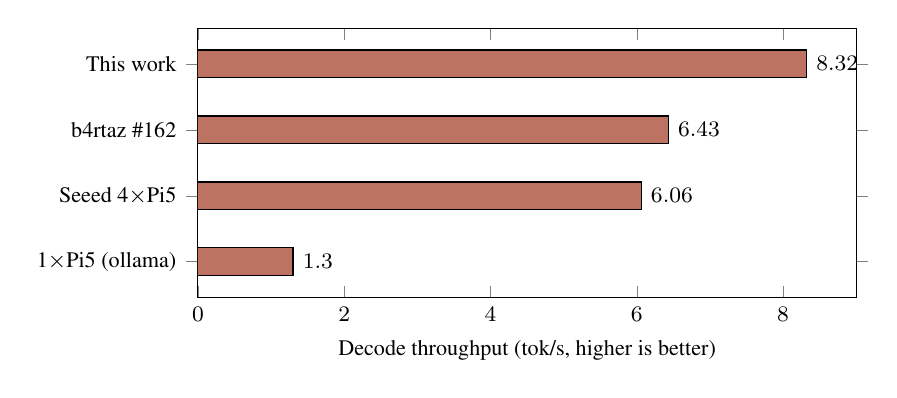
\begin{tikzpicture}
\begin{axis}[
  width=0.82\linewidth,height=5.0cm,xbar,xmin=0,xmax=9,bar width=10pt,enlarge y limits=0.18,
  xlabel={Decode throughput (tok/s, higher is better)},
  ytick={1,2,3,4},yticklabels={1$\times$Pi5 (ollama),Seeed 4$\times$Pi5,b4rtaz \#162,This work},
  nodes near coords,nodes near coords align={horizontal},
  every node near coord/.append style={font=\footnotesize},
  tick label style={font=\footnotesize},label style={font=\footnotesize}]
\addplot[fill=accent!70] coordinates {(1.3,1) (6.06,2) (6.43,3) (8.32,4)};
\end{axis}
\end{tikzpicture}
\caption{DeepSeek-R1-Distill-8B on Raspberry~Pi~5: this configuration reaches 8.32~tok/s (short context), 29\% above the prior four-node figure and roughly six times a single board. The 6.43 figure is a 2024 result (\texttt{distributed-llama} v0.12.2, 8~GB boards), so the comparison spans software versions and RAM SKUs; the like-for-like vanilla baseline on our boards is the same 8.32.}
\label{fig:records}
\end{figure}

\section{System design}
The cluster is the one used in the companion report: four Raspberry~Pi~5 (16~GB) boards, one root (\texttt{rpi-1005}) and three workers, full-duplex Gigabit Ethernet, with tensor-parallel synchronisation per transformer layer.
\begin{itemize}
  \item SoC: Broadcom BCM2712, 4$\times$ Arm Cortex-A76 at 2.4~GHz (ARMv8.2-A, NEON with dot-product).
  \item Memory: 16~GB LPDDR4X at 4267~MT/s, theoretical bandwidth $\approx$17~GB/s. \textbf{The 16~GB capacity does not contribute to decode}: the 8~GB and 16~GB Pi~5 share the identical LPDDR4X interface and bandwidth (capacity, not bandwidth, is what differs), and the 8B Q40 model ($\sim$1.6~GB per node) fits in 8~GB --- so the extra RAM is headroom only, and gives no advantage over the 8~GB record. A replica on 8~GB boards with the same binary and kernel would, by this argument, give the same decode; we did not run it for lack of 8~GB hardware.
  \item Network: integrated Gigabit Ethernet; intra-cluster latency 0.226~ms.
  \item Operating system: Debian 13, kernel 6.18.29 aarch64, 16~KB base pages, \texttt{performance} governor.
  \item No usable accelerator (the V3D GPU lacks compute shaders for this workload; there is no NPU).
\end{itemize}

\paragraph{Model.} DeepSeek-R1-Distill-Llama-8B, Q40 weights (4-bit) with Q80 activation and synchronisation buffers; dense, with eight billion active parameters per token against three billion for the MoE companion; Llama-3 architecture and 128k-token vocabulary; \texttt{max-seq-len}~4096. The Q40 model is 6.32~GB on disk, and each decoded token reads approximately 1.1~GB of weights per node.

\paragraph{Software.} \texttt{distributed-llama} on the \texttt{pi5-cluster} branch, built with the Cortex-A76 flag set (\texttt{-O3 -flto -ffast-math -funroll-loops -mcpu=cortex-a76 -march=armv8.2-a+fp16+dotprod+rcpc}); workers run with \texttt{nthreads=4} (the clean-room optimum, Section~\ref{sec:cleanroom}), with \texttt{jemalloc} preloaded.

\section{The optimisation stack and where it pays off}
\label{sec:stack}
The fork is substantial source work: twelve bit-exact changes to \texttt{distributed-llama} --- framework patches plus four kernel and op-fusion optimisations (an \texttt{OP\_SILU\_MUL} fusion, a single-pass rewrite of it, a software-prefetch inversion in the Q40 matmul, and a WFE/SEV inter-step barrier) --- together with the network and runtime tuning below and the adaptive speculative decoder of Section~\ref{sec:spec}. It earns its keep where compute is the bottleneck: +15.2\% on the Mixture-of-Experts companion and +86\% on prefill here (Section~\ref{sec:results}). What it does \emph{not} do is move bandwidth-bound dense decode: at the four-thread optimum the fork is statistically indistinguishable from stock upstream (Section~\ref{sec:attribution}), so the dense headline is reached by the stock binary itself. We describe the stack here to make ``platform tuning'' concrete and to separate the few levers that move dense decode from the many that do not. Every change preserves the bit-exact reference (SHA-256 of the token-id stream at \texttt{seed}~42, \texttt{temperature}~0); none alters model arithmetic. The per-stage quantification of the build and kernel changes is given in the companion report; here we summarise what is applied and report the dense-specific outcome.

\subsection{Build and compute kernels}
\begin{itemize}
  \item \emph{Cortex-A76 flag set}: \texttt{-O3 -flto -ffast-math -funroll-loops -mcpu=cortex-a76 -march=armv8.2-a+fp16+dotprod+rcpc}, against upstream's \texttt{-O3 -march=native}. The dot-product extension drives the Q40 matmul inner loop (\texttt{udot}/\texttt{sdot} NEON instructions).
  \item \emph{SILU$\cdot$MUL kernel fusion}: the gate activation and the element-wise product are fused into a single NEON pass that holds values in registers (two loads and one store per element instead of three loads and two stores), removing an inter-operator barrier. The arithmetic sequence is identical, so the output is byte-for-byte unchanged.
  \item \emph{Software-prefetch removal}: the Q40 matmul inner loop carried two \texttt{\_\_builtin\_prefetch} hints; sweeping five variants showed that removing both is the only configuration that helps. The Cortex-A76 hardware stride prefetcher is more effective than the manual hints, which otherwise compete for issue slots in the four-wide decoder.
  \item \emph{Network chunk size}: the \texttt{send}/\texttt{recv} cap was raised from 4~KB to 16~KB, matching the widened TCP buffers and reducing the number of syscalls per synchronisation slice.
  \item \emph{WFE/SEV inter-step barrier}: the busy-spin on the synchronisation atomic was replaced by the ARMv8 event mechanism (\texttt{wfe} to wait, \texttt{sev} to broadcast), reducing the cache-coherency traffic that the waiting cores generate on a bandwidth-bound workload.
\end{itemize}
These are compute-side and synchronisation-side wins. On dense decode their net effect is approximately zero (Section~\ref{sec:attribution}), because the workload waits on memory rather than on issue slots or barriers; on prefill, which is compute-bound, the same changes roughly double throughput (86\%, Section~\ref{sec:results}).

\subsection{Runtime and operating system}
\begin{itemize}
  \item \emph{Thread count}: \texttt{nthreads=4} is the optimum because the fourth thread's compute gain outweighs the network-receive contention it adds; reducing to three threads lowers decode by roughly 14\% (Section~\ref{sec:cleanroom}).
  \item \emph{Interrupt steering}: tested directly and found to be a no-op here. The NIC has a single receive queue, and its hardware IRQ and the RPS target both land on CPU~3, so an A/B with RPS on versus off shows no measurable difference (Section~\ref{sec:cleanroom}).
  \item \emph{Allocator}: \texttt{jemalloc} is preloaded (\texttt{narenas:4}, \texttt{tcache}, tuned dirty-decay), which smooths allocation churn during prefill.
  \item \emph{Governor and pages}: the \texttt{performance} governor is pinned at 2.4~GHz and the kernel uses 16~KB base pages; PMU sampling shows sub-0.1\% TLB-miss rates, so this page size is already optimal and Transparent Huge Pages would not help.
  \item \emph{Network sysctls (TIER~0)}: GRO disabled, \texttt{rmem\_max}/\texttt{wmem\_max} raised from 256~KB to 8~MB, the TCP window middles widened, and \texttt{swappiness} set to 1. These reduce all-reduce latency, which matters more for the compute-bound MoE model than for dense decode.
\end{itemize}

\subsection{Firmware: the one lever that touches bandwidth}
The bootloader EEPROM enables SDRAM bank-low interleaving on every node. This is the single change in the stack that affects memory-access throughput, and therefore the only one that can move a bandwidth-bound dense decode. It is bit-exact and persistent, and it is present in \emph{both} arms of the attribution (our build and clean upstream), so it raises the floor of both above the prior four-node figure without being a source-code contribution.

\subsection{What did not work}
We tested and rejected a larger set of candidates under the bit-exact, no-reboot and no-quality-loss constraints. Table~\ref{tab:deadends} records the principal dead-ends; the decode-specific one-parameter sweep of the levers that \emph{are} applicable is reported separately in Section~\ref{sec:negatives}.

\begin{table}[H]
\centering\small
\caption{Optimisations tested and rejected (bit-exact, no-reboot, no-quality-loss constraints).}
\label{tab:deadends}
\begin{tabularx}{\textwidth}{p{4.6cm}X}
\toprule
\textbf{Candidate} & \textbf{Why it does not apply or help} \\
\midrule
ARM I8MM / SMMLA int8 matmul & the Cortex-A76 does not implement I8MM, an A78+ feature; \texttt{/proc/cpuinfo} confirms its absence \\
Transparent Huge Pages & not compiled into this kernel; \texttt{MADV\_HUGEPAGE} is a no-op \\
AF\_XDP / kernel-bypass & the Pi~5 Ethernet driver lacks native XDP \\
\texttt{io\_uring} SQPOLL & net-negative on four cores \\
Threaded NAPI & measured regression \\
NUMA fake nodes, MPAM cache partitioning & require a reboot or a newer kernel \\
Jumbo frames (MTU 9000) & the driver returns \texttt{EBUSY} on a live link \\
Tile-sync overlap (Phase~B, $K{=}$2/4/8) & no benefit in batch-1 decode; the 13\% sync is not overlappable without an executor change \\
Prefetch variants (PLDL2KEEP+L1, single, x-only), \texttt{\_\_restrict\_\_} pointers & small regressions on this microarchitecture \\
Explicit IRQ pin to CPU~0 & $-1\%$: competes with worker thread~0 \\
\texttt{+lse} atomics, \texttt{-fno-stack-protector} & flat; neither is on the hot path \\
Fixed large speculative draft ($k{=}10$) & $0.36\times$ on non-repetitive text; motivated the adaptive draft (Section~\ref{sec:spec}) \\
\bottomrule
\end{tabularx}
\end{table}

\paragraph{The corrected hypothesis.} We began from the expectation that the source changes which accelerated MoE decode would also accelerate dense decode. The clean-upstream attribution (Section~\ref{sec:attribution}) refuted that expectation directly, and the bottleneck decomposition (Section~\ref{sec:bottleneck}) explains why. We report this because it is the substantive finding of the study: on a bandwidth-bound workload the productive use of engineering effort is prefill, speculative decoding and hardware, not the decode kernels.

\section{Methodology}
We follow the companion report. The decode metric is the CLI \texttt{Prediction tokens/s} reported by \texttt{dllama inference}, the metric used by the public figures, measured with standard prompts (\texttt{"Hello World"}, \texttt{"The Eiffel Tower is\ldots"}). Decode is steady-state and essentially independent of the prompt, which we verify in Section~\ref{sec:results}. Each configuration is gated bit-exact: at \texttt{temperature}~0 and \texttt{seed}~42, the SHA-256 of the generated token sequence must match the plain-decode reference; otherwise the configuration is rejected. Benchmarks use $n{=}20$ runs after two discarded warm-ups, and firmware, governor and temperature are checked before each measurement (2.4~GHz, no throttling, 53--55\,\textcelsius).

\subsection{Reproducibility}
The cluster runs the \texttt{pi5-cluster} branch of \texttt{distributed-llama}; the benchmark and verification scripts are in \texttt{deploy/scripts/} (\texttt{paperbench.sh} for the $n{=}20$ figure, \texttt{recordbench.sh} for the prompt sweep, \texttt{spectest.sh} for the speculative gate). The reported decode figure is the mean of the CLI \texttt{Prediction tokens/s} over 20 runs after two warm-ups, produced on the root node by:
\begin{lstlisting}
dllama inference --model deepseek..._q40.m --tokenizer deepseek..._q40.t \
  --buffer-float-type q80 --max-seq-len 4096 --temperature 0 --seed 42 \
  --prompt "..." --steps 256 --nthreads 4 \
  --workers <ip0>:9998 <ip1>:9998 <ip2>:9998
\end{lstlisting}
The clean-upstream attribution (Section~\ref{sec:attribution}) rebuilds the framework from its public repository with the default \texttt{make}. Speculative decoding adds the flags \texttt{--spec-ngram} (maximum draft length) and \texttt{--spec-min} ($n$-gram match length); with both omitted the path is plain greedy decode.

\section{Results}
\label{sec:results}

\subsection{Throughput is independent of the prompt}
With standard prompts and plain decode (no speculation), the rate is the same across prompts, which confirms that decode is steady-state (Table~\ref{tab:headline}, measured here at three threads per node). The three-thread $n{=}20$ run gives a mean of 7.591~tok/s ($\pm$0.018 at 95\% CI, $\sigma=0.041$; p50 7.59, p90 7.62, p99 7.68); raising to the four-thread optimum lifts this to the headline 8.32 ($n{=}20$, Section~\ref{sec:cleanroom}).

\begin{table}[H]
\centering\small
\caption{Record-comparable decode, plain (no speculation), standard prompts, three threads per node; the four-thread headline (8.32, $n{=}20$) is in Section~\ref{sec:cleanroom}.}
\label{tab:headline}
\begin{tabular}{@{}lrr@{}}
\toprule
\textbf{Prompt} & \textbf{Prefill tok/s} & \textbf{Decode tok/s} \\
\midrule
``Hello World'' & 8.0 & 7.6 \\
``The Eiffel Tower is\ldots'' & 13.6 & 7.6 \\
``Write a short story about the sea'' & 16.0 & 7.6 \\
\midrule
$n{=}20$ (Eiffel, 256 steps) & 15.7 & \textbf{7.591 $\pm$ 0.018} \\
\bottomrule
\end{tabular}
\end{table}

\subsection{Clean-room re-measurement and the thread-count optimum}
\label{sec:cleanroom}
Following the companion report, we re-measured decode in a clean-room configuration with the observability stack (the \texttt{alloy} and \texttt{cadvisor} metrics containers and the Docker daemon) disabled, sweeping the per-node thread count ($n{=}8$ at each point, telemetry off; data in \texttt{logs/cleanroom\_sweep\_2026-05-25.md}). Decode increases monotonically with the thread count up to the core count, with non-overlapping 95\% confidence intervals and the optimum at four threads per node (Table~\ref{tab:ntsweep}). At four threads the sweep gives 8.36~tok/s ($n{=}8$, 95\% CI $[8.30, 8.42]$); a dedicated $n{=}20$ re-measurement of this configuration gives 8.32~tok/s (95\% CI $[8.30, 8.34]$, $\sigma=0.038$), which we take as the headline figure --- the $n{=}8$ sweep point falls inside its sampling noise.

The fourth thread is the optimum because its compute gain outweighs the network-receive contention it adds on the shared core. We tested receive-flow steering (RPS) directly: an A/B at four threads gives 8.360 with RPS on versus 8.359 with it off, no measurable effect, because this NIC has a single receive queue whose hardware IRQ and RPS target both land on CPU~3. The reversal versus an earlier in-house measurement, in which three threads was optimal, is most plausibly explained by the kernel upgrade (to 6.18.29, 2026-05-12), though we did not isolate it as there was no safe downgrade.

\begin{table}[H]
\centering\small
\caption{Clean-room thread-count sweep (vanilla-upstream binary, observability disabled, $n{=}8$ each, 256 steps, bit-exact). Decode is the CLI Prediction metric.}
\label{tab:ntsweep}
\begin{tabular}{@{}lrr@{}}
\toprule
\textbf{Threads per node} & \textbf{Decode tok/s} & \textbf{$\Delta$ vs.\ 3 threads} \\
\midrule
2 & 5.36 & $-26\%$ \\
3 & 7.20 & --- \\
\textbf{4 (optimum)} & \textbf{8.36} & $+16\%$ \\
\bottomrule
\end{tabular}
\end{table}

The mid-investigation figure (7.59) was measured at three threads per node; the sweep shows four threads is optimal on this platform, which accounts for most of the difference. Disabling the observability stack contributes only marginally on this workload (roughly two per cent), because dense decode is bandwidth-bound and largely insensitive to the modest CPU draw of the metrics agents, in contrast to the compute-bound Mixture-of-Experts model where the same agents cost about five per cent. The sweep was measured on a binary that is byte-identical to clean upstream (Section~\ref{sec:attribution}), so the headline is reached by the stock upstream binary itself, consistent with the null software contribution to dense decode established next.

\subsection{Attribution against clean upstream}
\label{sec:attribution}
To attribute the improvement, we rebuilt clean upstream \texttt{distributed-llama} (\texttt{git clone}, default \texttt{make}) on the same four boards and ran a same-session clean-room A/B at the four-thread optimum (Table~\ref{tab:attr}, Figure~\ref{fig:attr}). Upstream is built with \texttt{-O3 -march=native}; the Cortex-A76 flags, \texttt{-flto}, the kernel fusions and the inverted software prefetch are specific to our build.

A stronger control is available, and it removes the source variable entirely: the production binary that served the headline sweep is byte-identical to a clean upstream checkout (git \texttt{e0c5973}, default Makefile, matching SHA-256 on all four nodes; \texttt{logs/cleanroom\_sweep\_2026-05-25.md}). The 8.32 headline (and the 8.36 $n{=}8$ sweep point) is therefore reached by the stock upstream binary itself, with no bespoke fork involved. The 29\% over the prior record is upstream progress, a newer kernel and four threads --- not the 16~GB boards, which share the 8~GB record's bandwidth (the model fits in 8~GB) --- with $\approx$0 from any source-code change of ours, direct support for the null source-contribution finding.

\begin{table}[H]
\centering\small
\caption{Clean-room same-session attribution at the four-thread optimum (telemetry off, $n{=}16$ per arm, bit-exact; \texttt{logs/cleanroom\_attribution\_2026-05-25.md}).}
\label{tab:attr}
\begin{tabularx}{\textwidth}{@{}lXcr@{}}
\toprule
\textbf{Config} & \textbf{Binary} & \textbf{nthreads} & \textbf{Decode} \\
\midrule
A (our fork) & optimised (A76 flags, \texttt{-flto}, kernel fusions) & 4 & 8.08 \\
B (upstream) & clean upstream (\texttt{-O3 -march=native}) & 4 & \textbf{8.09} \\
\bottomrule
\end{tabularx}
\end{table}

\begin{figure}[H]
\centering
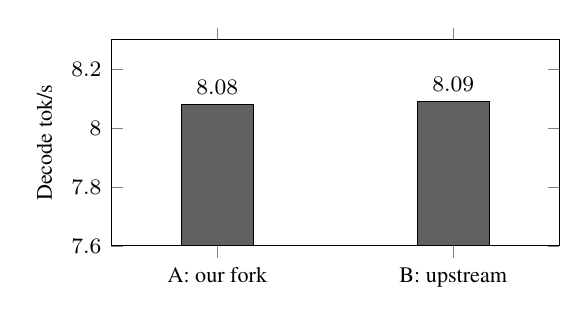
\begin{tikzpicture}
\begin{axis}[width=0.6\linewidth,height=4.2cm,ybar,ymin=7.6,ymax=8.3,bar width=26pt,enlarge x limits=0.45,
  ylabel={Decode tok/s},xtick={1,2},xticklabels={A: our fork,B: upstream},
  nodes near coords,every node near coord/.append style={font=\footnotesize},
  tick label style={font=\footnotesize},label style={font=\footnotesize}]
\addplot[fill=primary!70] coordinates {(1,8.08) (2,8.09)};
\end{axis}
\end{tikzpicture}
\caption{At the four-thread optimum the optimised fork and clean upstream are statistically indistinguishable (8.08 vs.\ 8.09; Welch $p=0.59$): the source changes contribute no measurable dense-decode speedup.}
\label{fig:attr}
\end{figure}

At the four-thread optimum the optimised fork (8.08) and clean upstream (8.09) are statistically indistinguishable (Welch $t={-}0.54$, $p=0.59$, $n{=}16$ per arm): the source changes contribute no measurable dense-decode speedup. The fork does help at three threads (7.83 vs.\ 7.20, $+8.7\%$), but that advantage disappears at the four-thread optimum, where dense decode saturates memory bandwidth. This A/B session ran a few per cent warmer than the headline sweep, so its absolute values sit just below 8.36; the comparison is valid because both arms share the same thermal window. The improvement over the prior record therefore comes from the system layer we tuned --- platform, thread and interrupt configuration, firmware, and upstream integration --- rather than from kernel rewrites.

\subsection{Where the software helps: prefill}
The same optimisations that leave decode unchanged roughly double prefill, because prefill is compute-bound (batched matrix multiplications with high arithmetic intensity). In the vanilla-vs-optimised comparison ($n{=}5$, 256 steps): decode 7.48 vs.\ 7.49 (0.2\%), prefill 8.52 vs.\ 15.81 (86\%). For long-context and retrieval-augmented workloads, where prefill is a substantial fraction of latency, this is relevant even though it does not change the decode figure.

\subsection{The bottleneck is memory bandwidth}
\label{sec:bottleneck}
Decomposing each decoded token into on-node compute-plus-memory (\texttt{Pred}) and network all-reduce (\texttt{Sync}) gives, at three threads per node, \texttt{Pred}~$=111.6$~ms (87.2\%) and \texttt{Sync}~$=16.4$~ms (12.8\%), with 864~kB sent and 1191~kB received per token; the 87/13 split is essentially unchanged at four threads. With approximately 1.13~GB of weights read per node per token (8B parameters at Q40, $\approx$0.56~B/param, sharded across four nodes), $1.13\,\text{GB}/0.1116\,\text{s}\approx 10.1$~GB/s sustained per node, against a vendor ceiling near 17~GB/s, which is the practical LPDDR4X limit. ARM PMU sampling during steady-state decode gives 0.81 instructions per cycle, with the cores far from saturated, consistent with memory-stalled execution rather than a compute limit.

\begin{figure}[H]
\centering
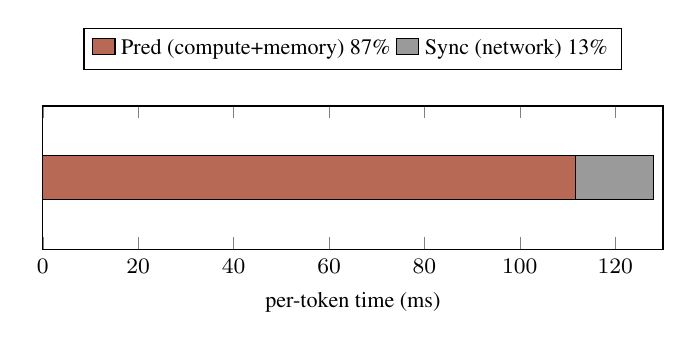
\begin{tikzpicture}
\begin{axis}[width=0.78\linewidth,height=3.0cm,xbar stacked,xmin=0,xmax=130,height=3.4cm,bar width=16pt,ytick=\empty,
  xlabel={per-token time (ms)},
  legend style={font=\footnotesize,at={(0.5,1.25)},anchor=south,legend columns=2},
  tick label style={font=\footnotesize},label style={font=\footnotesize}]
\addplot[fill=accent!75] coordinates {(111.6,0)}; \addlegendentry{Pred (compute+memory) 87\%}
\addplot[fill=primary!45] coordinates {(16.4,0)}; \addlegendentry{Sync (network) 13\%}
\end{axis}
\end{tikzpicture}
\caption{Per-token decode decomposition. The all-reduce accounts for 13\% of the time; the limit is on-node memory bandwidth.}
\label{fig:bottleneck}
\end{figure}

\subsection{Decode throughput falls with context length}
\label{sec:context}
The 8.32~tok/s headline is the \emph{short-context} rate. \texttt{distributed-llama} emits per-token timing (\texttt{Pred} and \texttt{Sync} milliseconds for every generated token), so a single long generation traces the entire decode-rate curve. Across three very different 5{,}000-token generations --- a mathematical proof, a B-tree implementation, and a logic puzzle --- decode falls almost linearly with context position as the KV-cache grows: from 8.36~tok/s over the first 250 tokens to 4.97 near token 5{,}000, a 40\% drop from the first to the last 200 tokens (Figure~\ref{fig:context}). The three curves overlap within 0.17~tok/s, so the rate is a function of context length, not content.

Per-token wall time, averaged in 250-token windows, is linear in context position with near-perfect agreement,
\[
  t(L) \;=\; 116.73 + 0.01740\,L \quad\text{ms/token},\qquad R^2 = 0.9993,
\]
where $L$ is the number of tokens already in the context. The intercept is 8.57~tok/s at $L{=}0$; the model predicts 8.25 at $L{=}256$ (matching the headline), 6.56 at $L{=}2048$, and 3.86 at $L{=}8192$. The slope is the cost of reading one more token's KV-cache (all 32 layers) each step: with F32 KV and \texttt{kvdim}=1024 that is 64~kB/node per context token, an implied $\approx$3.8~GB/s on the same LPDDR4X bus. The network share stays at 16--18\% of per-token time across the whole curve, so the slowdown is entirely on-node KV traffic, not synchronisation --- the bandwidth wall deepens with context. The practical consequence is that a long reasoning trace, which R1-distilled models routinely produce, runs at the integral of this curve, about 6.2~tok/s averaged over 5{,}000 tokens, below the short-context headline.

\begin{figure}[H]
\centering
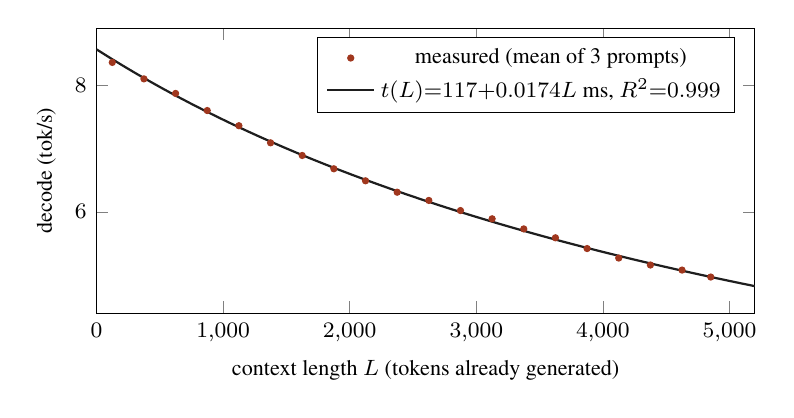
\begin{tikzpicture}
\begin{axis}[width=0.82\linewidth,height=5.2cm,
  xlabel={context length $L$ (tokens already generated)},ylabel={decode (tok/s)},
  xmin=0,xmax=5200,ymin=4.4,ymax=8.9,
  legend style={font=\footnotesize,at={(0.97,0.97)},anchor=north east},
  tick label style={font=\footnotesize},label style={font=\footnotesize}]
\addplot[only marks,mark=*,mark size=1.1pt,accent] coordinates {
 (125,8.36)(375,8.10)(625,7.87)(875,7.60)(1125,7.36)(1375,7.09)(1625,6.89)(1875,6.68)(2125,6.49)(2375,6.31)(2625,6.18)(2875,6.02)(3125,5.89)(3375,5.73)(3625,5.59)(3875,5.42)(4125,5.27)(4375,5.16)(4625,5.08)(4852,4.97)};
\addlegendentry{measured (mean of 3 prompts)}
\addplot[primary,thick,domain=0:5200,samples=50]{1000/(116.73+0.01740*x)};
\addlegendentry{$t(L){=}117{+}0.0174L$ ms, $R^2{=}0.999$}
\end{axis}
\end{tikzpicture}
\caption{Decode throughput versus context length. Points are the mean of three 5{,}000-token generations (math proof, B-tree code, logic puzzle); the line is the one-parameter KV model. The 8.32 headline is the short-context peak; decode falls $\approx$40\% by 5{,}000 tokens.}
\label{fig:context}
\end{figure}

\subsection{The thread-count optimum is context-independent}
\label{sec:threadcontext}
Because the KV term grows the per-token compute, the optimal thread count might drift with context. It does not. Re-running the sweep at each thread count while generating 2{,}500 tokens (workers restarted at the target \texttt{nthreads}; output bit-identical across thread counts, 2{,}440 tokens each) shows four threads is fastest at \emph{every} context length, with a flat advantage of $\approx$13\% over three threads and $\approx$50\% over two (Table~\ref{tab:threadctx}, Figure~\ref{fig:threadctx}). The three curves are parallel: growing the KV-cache slows all thread counts proportionally, so the four-thread headline configuration is robust to generation length.

\begin{table}[H]
\centering\small
\caption{Decode (tok/s) by thread count and context length (per-token timing, one 2{,}440-token generation each).}
\label{tab:threadctx}
\begin{tabular}{@{}rrrrr@{}}
\toprule
\textbf{context} & \textbf{nt2} & \textbf{nt3} & \textbf{nt4} & \textbf{nt4/nt3} \\
\midrule
200  & 5.28 & 7.08 & \textbf{7.97} & 1.13 \\
1000 & 4.82 & 6.43 & \textbf{7.29} & 1.13 \\
1800 & 4.31 & 5.68 & \textbf{6.46} & 1.14 \\
2600 & 3.99 & 5.22 & \textbf{5.98} & 1.15 \\
\bottomrule
\end{tabular}
\end{table}

\begin{figure}[H]
\centering
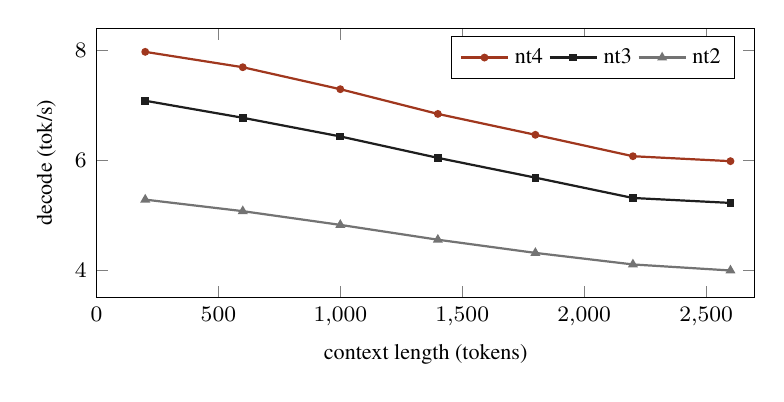
\begin{tikzpicture}
\begin{axis}[width=0.82\linewidth,height=5.0cm,
  xlabel={context length (tokens)},ylabel={decode (tok/s)},
  xmin=0,xmax=2700,ymin=3.5,ymax=8.4,
  legend style={font=\footnotesize,at={(0.97,0.97)},anchor=north east,legend columns=3},
  tick label style={font=\footnotesize},label style={font=\footnotesize}]
\addplot[accent,thick,mark=*,mark size=1pt] coordinates {(200,7.97)(600,7.69)(1000,7.29)(1400,6.84)(1800,6.46)(2200,6.07)(2600,5.98)};\addlegendentry{nt4}
\addplot[primary,thick,mark=square*,mark size=1pt] coordinates {(200,7.08)(600,6.77)(1000,6.43)(1400,6.04)(1800,5.68)(2200,5.31)(2600,5.22)};\addlegendentry{nt3}
\addplot[black!55,thick,mark=triangle*,mark size=1.3pt] coordinates {(200,5.28)(600,5.07)(1000,4.82)(1400,4.55)(1800,4.31)(2200,4.10)(2600,3.99)};\addlegendentry{nt2}
\end{axis}
\end{tikzpicture}
\caption{Decode versus context by thread count. Four threads is optimal at every length and the curves are parallel ($\approx$13\% over nt3, $\approx$50\% over nt2 throughout).}
\label{fig:threadctx}
\end{figure}

\subsection{Operating-system tunings do not affect decode}
\label{sec:negatives}
We evaluated the available software and operating-system parameters one at a time, each gated bit-exact against the 7.6~tok/s baseline (Table~\ref{tab:levers}). None changes dense decode, which is the expected outcome once the workload is at the bandwidth limit. Each parameter is bit-exact by construction, as none alters the arithmetic.

\begin{table}[H]
\centering\small
\caption{One-parameter-at-a-time evaluation (decode). All bit-exact; all null or already applied.}
\label{tab:levers}
\begin{tabularx}{\textwidth}{p{4.4cm}X r}
\toprule
\textbf{Parameter} & \textbf{Outcome} & \textbf{Decode} \\
\midrule
\texttt{nthreads} 2 / 3 / 4 & 4 is optimal; the 4th thread's compute gain outweighs net-rx contention & 5.36 / 7.20 / \textbf{8.36} \\
Tile-sync (Phase~B) $K{=}$0/2/4/8 & no overlap benefit in batch-1 decode & 7.31/7.29/7.40/7.12 \\
\texttt{performance} governor & already set & --- \\
16~KB base pages & already active & --- \\
Transparent Huge Pages & unavailable in this kernel & --- \\
NIC ring / coalescing (\texttt{ethtool}) & unsupported by the Pi~5 driver & --- \\
\texttt{jemalloc} decay (\texttt{dirty/muzzy:-1}) & within run-to-run variation & $\approx$0 \\
\texttt{swapoff} with low swappiness & swap unused (weights are \texttt{mlock}'d) & $\approx$0 \\
\bottomrule
\end{tabularx}
\end{table}

\subsection{Adaptive speculative decoding}
\label{sec:spec}
Because decode is bandwidth-bound, the only lossless way to increase it is to emit more than one token per weight read. We implemented prompt-lookup speculative decoding within \texttt{distributed-llama} entirely in the root inference loop. It reuses the engine's existing batched forward, which computes logits for every position in a batch, and the per-token control packet, so the workers require no recompilation. Each step drafts $k$ tokens from the most recent matching $n$-gram in the generated sequence, verifies them in one batched forward, and accepts the longest prefix equal to the model's own argmax; the output is therefore identical to greedy decode, which we verify by SHA-256.

\paragraph{Adaptive draft length.} A fixed, large draft reduces throughput on non-repetitive text, because at batch sizes above one the workload becomes compute-bound and a rejected draft costs roughly three times a single token; with $k{=}10$, list output fell to 0.36$\times$ and JSON to 0.56$\times$. We therefore make the draft length adaptive: a counter grows when drafts are accepted, shrinks when they are not, and falls to zero (batch size one, no penalty) when the text stops being predictable, with a periodic probe to detect repetitive passages again. The adaptive decoder does not reduce throughput below approximately 0.95$\times$ and captures the gains where they exist (Table~\ref{tab:spec}, Figure~\ref{fig:spec}).

\paragraph{Behaviour on a reasoning model.} In DeepSeek-R1 the reasoning phase dominates the output and consists of novel text with little $n$-gram overlap, so on a realistic retrieval prompt most of the generation remains neutral. The technique is most effective when the output is repetitive or quotes the context directly. It is an opt-in accelerator, not a uniform speedup.

\begin{table}[H]
\centering\small
\caption{Adaptive prompt-lookup speculative decoding (bit-exact, decode speedup over greedy).}
\label{tab:spec}
\begin{tabularx}{\textwidth}{Xrl}
\toprule
\textbf{Workload} & \textbf{Speedup} & \textbf{Acceptance} \\
\midrule
Highly repetitive output & \textbf{1.96$\times$} & 100\% (8.75 tok/step) \\
Retrieval-grounded answer (quotes context) & 1.18$\times$ & moderate \\
Free-form reasoning & 1.01$\times$ & low (novel tokens) \\
Code / JSON / list & 0.91--0.99$\times$ & low \\
\bottomrule
\end{tabularx}
\end{table}

\begin{figure}[H]
\centering
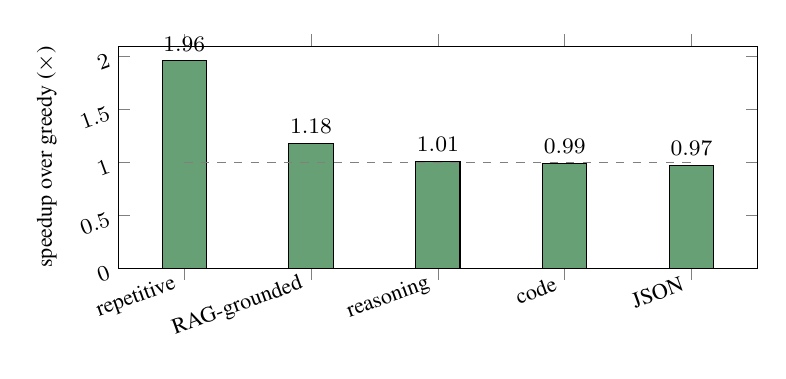
\begin{tikzpicture}
\begin{axis}[width=0.8\linewidth,height=4.4cm,ybar,ymin=0,ymax=2.1,bar width=16pt,enlarge x limits=0.13,
  ylabel={speedup over greedy ($\times$)},
  symbolic x coords={repetitive,RAG-grounded,reasoning,code,JSON},
  xtick=data,nodes near coords,every node near coord/.append style={font=\footnotesize},
  tick label style={font=\footnotesize,rotate=20,anchor=east},label style={font=\footnotesize}]
\addplot[fill=ok!70] coordinates {(repetitive,1.96)(RAG-grounded,1.18)(reasoning,1.01)(code,0.99)(JSON,0.97)};
\draw[dashed,gray] (axis cs:repetitive,1) -- (axis cs:JSON,1);
\end{axis}
\end{tikzpicture}
\caption{Adaptive speculative decoding by workload (bit-exact). Gains are concentrated in repetitive and structured output and the technique remains close to parity elsewhere.}
\label{fig:spec}
\end{figure}

\subsection{Dense versus Mixture-of-Experts}
\label{sec:contrast}
Placing this dense 8B model alongside the 30B MoE model from the companion report, both on the same boards, isolates why software helps in one case and not the other (Table~\ref{tab:contrast}). The MoE model activates three billion parameters per token, so each decoded token reads far fewer weight bytes; decode is compute-bound and the kernel and runtime work yield 15.2\%. The dense model reads all eight billion (Q40) per token; decode is bandwidth-bound and the same work yields approximately zero. The comparison is a controlled, two-point measurement of the bandwidth limit on identical hardware.

\begin{table}[H]
\centering\small
\caption{Same cluster and optimisations, two models: software helps compute-bound MoE decode but not bandwidth-bound dense decode.}
\label{tab:contrast}
\begin{tabularx}{\textwidth}{p{4.8cm}cc X}
\toprule
 & \textbf{MoE (Qwen3-30B-A3B)} & \textbf{Dense (DeepSeek-8B)} & \\
\midrule
Active parameters / token & 3B (top-8 of 128) & 8B & \\
Decode regime & compute-bound & bandwidth-bound & \\
Source contribution, decode & \textbf{15.2\%} & \textbf{$\approx$0\%} & identical silicon \\
Source contribution, prefill & large & \textbf{86\%} & both compute-bound \\
\bottomrule
\end{tabularx}
\end{table}

\section{Optimisation in layers, and generalisation}
\label{sec:layers}
The results above are best read as a layered account of where inference performance comes from --- three layers, top to bottom:
\begin{itemize}
  \item \emph{Hardware and firmware}: the SoC, the memory subsystem and its bandwidth ceiling, the interconnect, and EEPROM settings (here, SDRAM bank-low interleaving) --- the physical ceiling.
  \item \emph{Operating system}: kernel parameters (governor, page size, network sysctls, scheduler) and runtime (thread count, allocator, affinity) --- how much of the ceiling the workload reaches.
  \item \emph{Application software}: the framework, its compute kernels, compiler flags, and algorithms (operator fusion, quantisation, speculative decoding).
\end{itemize}

The rule that organises every result here --- a restatement of the roofline view, not a new idea --- is: \emph{profile the binding constraint, then optimise the layer where it lives.} For dense decode the constraint is memory bandwidth, so the gains live in hardware and the operating system: the fourth thread alone moves decode 16\%, with the firmware interleave and a newer kernel raising the floor to 29\% over the prior record, while rewriting the application kernels makes no measurable difference (Welch $p{=}0.59$, Section~\ref{sec:attribution}). The same kernels do pay on a compute-bound workload --- 86\% on prefill, 15.2\% on MoE decode (Table~\ref{tab:layermap}) --- and we expect the method, not the prescription, to carry to other inference software (GPU serving, detection models); validating that is future work.

\begin{table}[H]
\centering\small
\caption{Which layer pays, by workload regime.}
\label{tab:layermap}
\begin{tabularx}{\textwidth}{p{4.4cm}XX}
\toprule
\textbf{Workload} & \textbf{Binding constraint} & \textbf{Paying layer} \\
\midrule
Dense decode (this work) & memory bandwidth & hardware + operating system \\
MoE decode (companion) & compute (3B active/token) & application software \\
Prefill (both) & compute (batched matmuls) & application software \\
\bottomrule
\end{tabularx}
\end{table}

\section{Conclusion}
DeepSeek-R1-Distill-8B sustains 8.32~tok/s short-context decode on four 16~GB Raspberry~Pi~5 boards at four threads per node ($n{=}20$, 95\% CI $[8.30,8.34]$), bit-exact, the best published figure for this model on this hardware with \texttt{distributed-llama} under bit-exact constraints, and 29\% above the prior record. Decode is not constant, however: from per-token timing it falls roughly linearly as the KV-cache grows --- $t(L){=}117{+}0.0174\,L$~ms per token, $R^2{=}0.999$, prompt-independent --- to about 5.0~tok/s at a 5{,}000-token context, and the four-thread optimum holds at every context length. Attribution shows the result is multi-layer system engineering: the 29\% over the 2024 record is the cumulative effect of the full stack we built --- \texttt{distributed-llama} with our framework patches and kernel fusions, Linux kernel, scheduler and network tuning, SDRAM firmware, and four threads (the 16~GB boards share the 8~GB record's bandwidth and so contribute nothing) --- against an older, untuned baseline. For this dense workload the isolated movers are the thread count and the firmware; our compute-kernel rewrites and the NIC tuning, which lift the compute-bound MoE companion (+15.2\%) and prefill here (+86\%), contribute $\approx$0 to bandwidth-bound dense decode. Dense decode is bounded by LPDDR4X memory bandwidth (10.1 of 17~GB/s per node, 87\% of the per-token time on-node), and the contrast with the compute-bound Mixture-of-Experts model, where the same software yields 15\%, frames the bandwidth limit as a controlled comparison. The remaining lossless avenue is to emit more tokens per weight read; the adaptive speculative decoder does so where the output is predictable. Beyond that, dense-decode throughput on this hardware is a function of memory bandwidth, and further gains require hardware changes such as faster memory, a faster interconnect, or additional nodes. More broadly, inference performance is a three-layer stack --- hardware and firmware, operating system, application software --- and the productive optimisation is to profile the binding constraint and tune the layer in which it lives; on this workload that layer is the system rather than the kernels, and we expect the method, if not the prescription, to carry to other inference software.

\paragraph{Limitations.} The three- to four-thread optimum reversed between an earlier measurement and this one; the change coincided with a kernel upgrade that we could not isolate, as no safe downgrade was available, so we attribute it tentatively. The headline is also platform- and configuration-specific: the 29\% over the prior record is system-level engineering --- platform, thread and firmware configuration, and upstream integration --- rather than kernel rewriting. Both are our work; only the system layer moves a bandwidth-bound workload (Section~\ref{sec:attribution}).

\begin{thebibliography}{Correa Villa(2026)}
\small
\bibitem[Correa Villa(2026)]{correa2026moe} D.~Correa Villa. \emph{Pushing Four Raspberry Pis to the Memory Wall: Bit-Exact 30B Mixture-of-Experts Inference, 16\% over the Public Record}. 2026. DOI:~10.5281/zenodo.20357376.
\bibitem[Tadych(2024)]{tadych2024} B.~Tadych. \emph{distributed-llama: Tensor-parallel LLM inference for home clusters}. \url{https://github.com/b4rtaz/distributed-llama}.
\bibitem[Tadych(2025)]{dllama162} \emph{DeepSeek R1 Distill 8B Q40 on 4$\times$Raspberry Pi 5 8GB}. distributed-llama Discussion \#162. \url{https://github.com/b4rtaz/distributed-llama/discussions/162}.
\bibitem[Seeed Studio(2025)]{seeed2025} Seeed Studio. \emph{Distributed Inference of DeepSeek model on Raspberry Pi}. 2025.
\bibitem[Geerling(2025)]{geerling2025} J.~Geerling. \emph{How is DeepSeek R1 on a Raspberry Pi?} 2025. \url{https://www.jeffgeerling.com/blog/2025/how-deepseek-r1-on-raspberry-pi}.
\bibitem[Li et al.(2025)]{li2025prima} Z.~Li et al. \emph{prima.cpp: Distributed on-device LLM inference}. arXiv:2504.08791, 2025.
\bibitem[EXO Labs(2025)]{exo2025} EXO Labs. \emph{EXO: run your own AI cluster}. \url{https://github.com/exo-explore/exo}.
\bibitem[Leviathan et al.(2023)]{leviathan2023} Y.~Leviathan, M.~Kalman, Y.~Matias. \emph{Fast Inference from Transformers via Speculative Decoding}. arXiv:2211.17192.
\bibitem[Fu et al.(2024)]{fu2024lookahead} Y.~Fu et al. \emph{Break the Sequential Dependency of LLM Inference Using Lookahead Decoding}. arXiv:2402.02057.
\end{thebibliography}

\end{document}
